\documentclass[11pt]{article}

\usepackage[margin=1in]{geometry}
\usepackage{amsmath,amssymb,amsthm,mathtools}
\usepackage{bm}
\usepackage{xcolor}
\usepackage{booktabs}
\usepackage{enumitem}
\usepackage{tikz}
\usepackage{pgfplots}
\pgfplotsset{compat=1.17}
\usetikzlibrary{arrows.meta,positioning,calc}
\usepackage[ruled,vlined,linesnumbered]{algorithm2e}
\usepackage[round]{natbib}
\usepackage[colorlinks=true,linkcolor=blue!55!black,citecolor=teal!60!black,urlcolor=blue!55!black]{hyperref}

% ---------------------------------------------------------------------------
\theoremstyle{plain}
\newtheorem{theorem}{Theorem}
\newtheorem{proposition}[theorem]{Proposition}
\newtheorem{lemma}[theorem]{Lemma}
\newtheorem{corollary}[theorem]{Corollary}
\theoremstyle{definition}
\newtheorem{definition}[theorem]{Definition}
\newtheorem{assumption}[theorem]{Assumption}
\theoremstyle{remark}
\newtheorem{remark}[theorem]{Remark}

\DeclareMathOperator*{\argmax}{arg\,max}
\DeclareMathOperator*{\argmin}{arg\,min}
\DeclareMathOperator{\E}{\mathbb{E}}
\DeclareMathOperator{\Var}{Var}
\newcommand{\R}{\mathbb{R}}
\newcommand{\Xsp}{\mathcal{X}}
\newcommand{\X}{\mathcal{X}}
\newcommand{\Y}{\mathcal{Y}}
\newcommand{\Dens}{\mathcal{D}}
\newcommand{\Leafset}{\Lambda}
\newcommand{\inner}[2]{\langle #1,\, #2\rangle}
\newcommand{\eps}{\varepsilon}
\newcommand{\jpt}{\textsc{jpt}}
\newcommand{\jptforest}{\textsc{JPTForest}}
\newcommand{\likeboost}{\textsc{JPTLikelihoodBoost}}
\newcommand{\jptboost}{\textsc{JPTBoost}}
\newcommand{\mixture}{\textsc{MixtureJPT}}

% Consistent colour palette for the experimental bar charts.
\definecolor{cJPT}{HTML}{4C72B0}
\definecolor{cForest}{HTML}{55A868}
\definecolor{cBoost}{HTML}{C44E52}
\definecolor{cGBM}{HTML}{8172B3}

\title{\textbf{Ensemble Joint Probability Trees:\\[2pt]
Valid Joint Densities and Full Probabilistic Inference\\
for Bagged and Boosted Density Trees}}

\author{Daniel Nyga\\[2pt]
\small Institute for Artificial Intelligence, University of Bremen}
\date{Draft --- for review}

\begin{document}
\maketitle

\begin{abstract}
Joint Probability Trees (JPTs) are tree-structured estimators of a
\emph{full joint distribution} $P(\mathbf{X})$ over mixed numeric, integer
and symbolic variables, learned once and queried for arbitrary
conditionals, marginals, most-probable explanations and likelihoods.
A single JPT is a low-variance but high-bias estimator; the standard
remedies are \emph{bagging} and \emph{boosting}. This paper develops both
for JPTs with two engineering requirements as its guiding thread:
\emph{(R1)} the ensemble must itself be a fully valid, normalised joint
probability density, and \emph{(R2)} every inference algorithm of the
single tree---likelihood, conditional queries, posterior marginals,
expectation, most-probable explanation, conditioning, and
sampling---must translate to the ensemble. We show that both the bagged
ensemble \jptforest{} and the boosted ensemble \likeboost{} are finite
convex mixtures of JPTs and prove that such mixtures are valid joints with
no partition function: bagging by construction, boosting because the
greedy additive update $P_t=(1-\alpha_t)P_{t-1}+\alpha_t C_t$ unrolls into
an explicit convex combination whose weights sum to one. The boosting rule
itself is principled: it is exactly Frank--Wolfe ascent of the empirical
joint log-likelihood, with inverse-density reweighting as the component
oracle and a concave line search for $\alpha_t$. We then derive the
complete inference calculus of the ensemble: unconditional queries
distribute linearly over the members; conditional queries require the
evidence-adjusted \emph{responsibilities} $r_m(e)\propto w_m P^{(m)}(e)$;
conditioning an ensemble yields again an ensemble of JPTs (closure under
conditioning); MPE is computed by member-wise candidate generation with
mixture re-scoring, a lower bound that is exact in natural special cases;
and sampling is ancestral. Every formula corresponds one-to-one to a
method of the published implementation. A third, discriminative variant
(\jptboost) is included for maximal point accuracy; we state precisely why
it---and only it---gives up the joint density. A cross-validated study on
six standard datasets corroborates the design: bagging and likelihood
boosting consistently raise the held-out joint log-likelihood over a
single JPT, the discriminative variant closes most of the accuracy gap to
gradient-boosted baselines, and the generative ensembles answer the same
prediction queries as a by-product of a full joint.
\end{abstract}

% ===========================================================================
\section{Introduction}
\label{sec:intro}

A Joint Probability Tree \citep{nyga2023jpt} represents a joint
distribution $P(\mathbf{X})$ over a set of random variables
$\mathbf{X}=(X_1,\dots,X_D)$ on a problem space $\Xsp$ by recursively
partitioning $\Xsp$ with axis-aligned, univariate splits and placing a
simple factored distribution in each leaf. A tree structure
$T:\Xsp\mapsto\Leafset$ maps each point to one of $N$ leaves
$\Leafset=\{\lambda_1,\dots,\lambda_N\}$, an auxiliary variable $L$
indicates the leaf, and the joint factorises as
\begin{equation}
\label{eq:jpt-intro}
P(\mathbf{X}=\mathbf{x})
\;=\;\sum_{\lambda\in\Leafset} P(L=\lambda)\,
\prod_{i=1}^{D} P\!\left(X_i=x_i \mid L=\lambda\right).
\end{equation}
Unlike a discriminative decision tree or a gradient-boosted regressor, a
JPT is learned \emph{once} and then answers \emph{any} probabilistic query
over its variables: conditionals $P(\mathbf{Q}\mid\mathbf{E})$ for any
choice of query $\mathbf{Q}$ and evidence $\mathbf{E}$, marginals under
missing variables, most-probable explanations, exact likelihoods for
anomaly scoring, and i.i.d.\ sampling. This ``train once, query anything''
contract is the defining strength of the formalism and the property every
extension must be measured against.

The price of that generality is statistical: a single piecewise-constant
tree is a high-bias estimator. In the cross-validated study of
\S\ref{sec:experiments}, a single JPT trails gradient-boosted
discriminative baselines on every dataset. The natural remedy is to
\emph{ensemble} JPTs:
bagging \citep{breiman1996bagging,breiman2001rf} to remove variance, and
boosting to remove bias. But an ensemble of JPTs is only useful if it
keeps the contract that makes JPTs worth using in the first place. We
therefore impose two requirements up front and let them drive the entire
construction:

\begin{description}[leftmargin=1.6em,style=nextline]
\item[(R1) The ensemble is a valid joint density.] The combined model
$\bar P$ must be non-negative and integrate to one over the mixed
numeric/symbolic space---not approximately, not after renormalisation,
but by construction. Both the bagged and the boosted ensemble must
satisfy this.
\item[(R2) Every inference algorithm translates.] Likelihood
(\texttt{likelihood}, \texttt{pdf}), conditional queries
(\texttt{infer}), posterior marginals (\texttt{posterior}), expectation
(\texttt{expectation}), most-probable explanation (\texttt{mpe}),
conditioning (\texttt{conditional\_jpt}) and sampling (\texttt{sample})
must be available on the ensemble with well-defined semantics that reduce
to the single-tree semantics for an ensemble of size one.
\end{description}

\paragraph{Contributions.}
\begin{enumerate}[leftmargin=1.6em]
\item We show that a JPT is a \emph{self-normalised disjoint-support
mixture} and that any finite convex combination of JPTs over a shared
variable domain is again a normalised joint, with no partition function
(\S\ref{sec:jpt}, Prop.~\ref{prop:mixture-closed}). This settles (R1) for
bagging immediately (\S\ref{sec:bagging}).
\item We settle (R1) for boosting (\S\ref{sec:likeboost}): the greedy
additive update $P_t=(1-\alpha_t)P_{t-1}+\alpha_t C_t$ unrolls into an
explicit convex combination $\sum_t\beta_t C_t$ with $\beta_t\ge0$,
$\sum_t\beta_t=1$ (Prop.~\ref{prop:boost-valid}), so the boosted model is
a valid joint at every round. The update is not a heuristic: it is exactly
Frank--Wolfe ascent of the empirical joint log-likelihood, with
inverse-density reweighting as the component-training oracle and a
one-dimensional concave line search for $\alpha_t$ (Thm.~\ref{thm:fw}).
\item We derive the complete inference calculus of the ensemble
(\S\ref{sec:inference}), settling (R2): likelihood and all unconditional
queries distribute linearly (Prop.~\ref{prop:uncond}); conditional
queries and posteriors require the evidence-adjusted responsibilities
$r_m(e)\propto w_m P^{(m)}(e)$ and we show the naive weight-preserving
average is wrong (Prop.~\ref{prop:cond}); ensembles are \emph{closed
under conditioning}---the conditional of an ensemble JPT is again an
ensemble JPT (Prop.~\ref{prop:closure}); MPE is computed by member-wise
candidate generation with mixture re-scoring
(Alg.~\ref{alg:mpe}, Prop.~\ref{prop:mpe}); sampling is ancestral. Each
formula maps one-to-one to a method of the implementation.
\item We include a third, discriminative variant, \jptboost{}, for
maximal point-prediction accuracy, and state precisely why it---and only
it---forfeits the joint: additive boosting of a \emph{joint} density
would require an intractable partition function, whereas conditioning
collapses that normaliser to the target variable alone
(\S\ref{sec:gbm}).
\item We validate the design in a cross-validated study on six standard
datasets (\S\ref{sec:experiments}), with every number reproduced from
the public API of the published implementation.
\end{enumerate}

% ===========================================================================
\section{Joint Probability Trees and their mixtures}
\label{sec:jpt}

\paragraph{Data space and base measure.}
Let $\Xsp=\Xsp_1\times\cdots\times\Xsp_D$ be the space of all modelled
variables, with a fixed reference measure $\mu$---Lebesgue on numeric axes,
counting measure on symbolic / integer axes, products thereof on mixed
spaces. A \emph{density} (we use the term for the joint $P$ throughout,
mass or density according to the axis) is a measurable
$P:\Xsp\to\R_{\ge 0}$ with $\int_\Xsp P\, d\mu = 1$. Write $\Dens$ for the
convex set of densities on $\Xsp$ w.r.t.\ $\mu$. For prediction we
partition the variables into evidence/features and target,
$\mathbf{X}=(\mathbf{x},\mathbf{y})$, and write a generic point $z=
(\mathbf{x},\mathbf{y})$. Given a sample $D=\{z_i\}_{i=1}^n$, the empirical
mean log-likelihood of a density is
\begin{equation}
\label{eq:LL}
\mathcal{L}(P)\;=\;\frac{1}{n}\sum_{i=1}^n \log P(z_i).
\end{equation}

\paragraph{The tree as a leaf mixture.}
A JPT over $\mathbf{X}$ is a tree $T$ whose internal nodes each test one
variable against a threshold (numeric / integer) or a value subset
(symbolic). A leaf $\lambda\in\Leafset$ owns the cell
$C_\lambda\subseteq\Xsp$ of points whose decision path ends at $\lambda$;
the cells are disjoint and cover $\Xsp$,
\[
C_\lambda \cap C_{\lambda'} = \emptyset \ (\lambda\neq\lambda'),
\qquad \bigcup_{\lambda\in\Leafset} C_\lambda = \Xsp .
\]
Each leaf carries a \emph{factored} local distribution---a product of
per-variable univariate distributions,
\begin{equation}
\label{eq:leaf}
P(\mathbf{X}=\mathbf{x}\mid L=\lambda)\;=\;
\prod_{i=1}^{D} P(X_i=x_i\mid L=\lambda),
\end{equation}
each factor a univariate density/mass on its axis cell and self-normalised
there. The leaf prior $P(L=\lambda)$ is the fraction of training mass
routed to $\lambda$, so $\sum_\lambda P(L=\lambda)=1$, and the JPT
distribution is the disjoint-support mixture~\eqref{eq:jpt-intro}.

\begin{proposition}[Self-normalisation]
\label{prop:jpt-norm}
If each factor in \eqref{eq:leaf} integrates to $1$ over its axis cell and
$\sum_\lambda P(L=\lambda)=1$, then the JPT $P$ of \eqref{eq:jpt-intro}
lies in $\Dens$.
\end{proposition}
\begin{proof}
By Fubini over the product axes, $\int_{C_\lambda}P(\cdot\mid L{=}\lambda)
\,d\mu=\prod_i\int P(X_i\mid L{=}\lambda)\,d\mu_i = 1$. The cells are
disjoint, so $\int_\Xsp P\,d\mu=\sum_\lambda P(L{=}\lambda)
\int_{C_\lambda}P(\cdot\mid L{=}\lambda)\,d\mu=\sum_\lambda P(L{=}\lambda)
= 1$. Non-negativity is inherited factorwise.
\end{proof}

The point of Proposition~\ref{prop:jpt-norm} for ensembling is that
normalisation is \emph{structural}, not the result of dividing by an
integral. This is what survives convex combination:

\begin{proposition}[Mixtures of JPTs are valid joints]
\label{prop:mixture-closed}
Let $P^{(1)},\dots,P^{(M)}\in\Dens$ be JPTs over a common variable domain
$\mathbf{X}$ and measure $\mu$, and let $w\in\Delta^{M-1}$ be a weight
vector on the simplex. Then
\[
\bar P(z)\;=\;\sum_{m=1}^M w_m\, P^{(m)}(z)
\]
is a density on $\Xsp$: $\bar P\ge0$ and $\int_\Xsp\bar P\,d\mu=1$.
\end{proposition}
\begin{proof}
$\bar P\ge 0$ as a non-negative combination of non-negative functions, and
$\int\bar P\,d\mu=\sum_m w_m\int P^{(m)}d\mu=\sum_m w_m=1$.
\end{proof}

\begin{remark}[No partition function]
\label{rem:no-Z}
Proposition~\ref{prop:mixture-closed} is the structural reason a
\emph{mixture} ensemble of JPTs is free of the normalisation cost that
sinks \emph{product}-style density combination. A product-of-experts
$\bar P\propto\prod_m (P^{(m)})^{\beta_m}$ requires the partition function
$Z=\int\prod_m (P^{(m)})^{\beta_m}d\mu$, an integral over all of $\Xsp$
with no closed form for tree densities. A convex mixture has $Z\equiv 1$.
Every generative ensemble we build---bagging and likelihood
boosting---is a mixture for exactly this reason.
\end{remark}

In the implementation, the mixture is realised by the base class
\mixture{}, which holds the members $\{P^{(m)}\}_{m=1}^M$ and the weight
vector $w$, and carries the entire query surface derived in
\S\ref{sec:inference}. \jptforest{} and \likeboost{} are training
strategies on top of this base: they differ \emph{only} in how members
and weights are produced, never in what the resulting object \emph{is}---a
finite convex mixture of JPTs, hence by Proposition~\ref{prop:mixture-closed}
a fully valid joint probability distribution.

% ===========================================================================
\section{Bagging: \jptforest}
\label{sec:bagging}

The bagged ensemble fixes $w_m=1/M$ and trains each $P^{(m)}$ on an
independent bootstrap resample $D^{(m)}$ of $D$:
\begin{equation}
\label{eq:bag}
P^{\jptforest}(z)\;=\;\frac1M\sum_{m=1}^M P^{(m)}(z).
\end{equation}

\begin{corollary}[\jptforest{} is a valid joint]
\label{cor:bag-valid}
Each member is a JPT, hence in $\Dens$ (Prop.~\ref{prop:jpt-norm}); the
uniform weights lie on the simplex; so $P^{\jptforest}\in\Dens$ by
Proposition~\ref{prop:mixture-closed}. Requirement (R1) holds by
construction, at every ensemble size $M$.
\end{corollary}

The statistical role of bagging is \emph{variance reduction}, and the
mechanism is the classic one:

\begin{proposition}[Variance reduction of the bagged query]
\label{prop:bag-var}
Fix a query functional $T(P)=\E_P[g\mid\mathbf{x}]$ (e.g.\ a leaf-routed
conditional mean) that is approximately linear in the leaf statistics, and
let $\hat T^{(m)}=T(P^{(m)})$ be the per-member estimates with common
variance $\sigma^2$ and average pairwise correlation $\rho$ across
bootstrap members. The bagged estimate
$\bar T=\frac1M\sum_m \hat T^{(m)}$ has variance
\[
\Var(\bar T)\;=\;\rho\,\sigma^2 \;+\; \frac{1-\rho}{M}\,\sigma^2
\;\xrightarrow[M\to\infty]{}\; \rho\,\sigma^2 .
\]
\end{proposition}
\begin{proof}
Standard: $\Var\!\big(\frac1M\sum_m \hat T^{(m)}\big)=\frac1{M^2}
\big(M\sigma^2 + M(M-1)\rho\sigma^2\big)=\rho\sigma^2+\frac{1-\rho}{M}
\sigma^2$.
\end{proof}

Bagging removes the de-correlated part of the leaf-estimate variance,
which is large for high-variance greedy trees, but leaves the common bias
untouched. Since the members are independent given the data, training
parallelises trivially across processes. The remaining gap to additive
ensembles is bias, which is the province of boosting.

% ===========================================================================
\section{Boosting: \likeboost}
\label{sec:likeboost}

The boosted ensemble grows the mixture greedily. Starting from a single
tree $P_0=C_0$ trained on $D$, round $t$ trains a new component $C_t$ on
data reweighted toward the points the current mixture explains worst and
mixes it in with a step size $\alpha_t$:
\begin{equation}
\label{eq:boost-update}
P_t \;=\; (1-\alpha_t)\,P_{t-1} \;+\; \alpha_t\, C_t,
\qquad \alpha_t\in[0,1] .
\end{equation}

\subsection{The boosted model is a valid joint at every round}

The update \eqref{eq:boost-update} interpolates between two densities, so
validity is preserved round by round; unrolling the recursion makes the
mixture weights explicit and shows the boosted model is exactly the same
kind of object as the bagged one.

\begin{proposition}[\likeboost{} is a valid joint]
\label{prop:boost-valid}
Let $P_T$ be produced by \eqref{eq:boost-update} from JPT components
$C_0,\dots,C_T\in\Dens$ with steps $\alpha_1,\dots,\alpha_T\in[0,1]$
(and $\alpha_0\coloneqq1$). Then
\[
P_T \;=\; \sum_{t=0}^{T} \beta_t\, C_t,
\qquad
\beta_t \;=\; \alpha_t \prod_{s=t+1}^{T} (1-\alpha_s),
\]
with $\beta_t\ge 0$ and $\sum_{t=0}^T\beta_t=1$. Hence $P_T$ is a finite
convex mixture of JPTs and, by Proposition~\ref{prop:mixture-closed}, a
fully valid normalised joint distribution---at every round $T$, for every
choice of the steps. Requirement (R1) holds by construction.
\end{proposition}
\begin{proof}
Induction on $T$. For $T=0$, $P_0=C_0$ and $\beta_0=\alpha_0=1$. Assume
$P_{T-1}=\sum_{t<T}\beta'_t C_t$ with $\beta'_t=\alpha_t\prod_{s=t+1}^{T-1}
(1-\alpha_s)$ summing to one. Then
$P_T=(1-\alpha_T)\sum_{t<T}\beta'_t C_t+\alpha_T C_T$, whose coefficients
are $\beta_t=(1-\alpha_T)\beta'_t$ for $t<T$ and $\beta_T=\alpha_T$,
matching the stated product formula, all non-negative, and summing to
$(1-\alpha_T)\cdot 1+\alpha_T=1$.
\end{proof}

Note what Proposition~\ref{prop:boost-valid} does \emph{not} require: no
renormalisation step, no partition function, no constraint coupling the
components. The implementation maintains exactly the weights $\beta_t$
(it rescales the stored weight vector by $(1-\alpha_t)$ and appends
$\alpha_t$ each round), so the serialised model is a plain
\mixture{}---indistinguishable, as a distribution object, from a forest
with non-uniform weights. Every inference result of \S\ref{sec:inference}
therefore applies verbatim to the boosted model.

\subsection{Why this boosting rule: Frank--Wolfe on the joint likelihood}
\label{sec:fw}

The specific choices of reweighting and step size are not heuristics; they
are the two moves of Frank--Wolfe (conditional-gradient) ascent
\citep{frankwolfe1956,jaggi2013fw} applied to the empirical joint
log-likelihood $\mathcal{L}$ of \eqref{eq:LL} over the convex hull
$\mathcal{C}=\operatorname{conv}(\mathcal{A})$ of the set $\mathcal{A}$ of
JPTs trainable from (reweighted) data. We record the statement; the
reader interested only in using the ensemble may skip to
\S\ref{sec:inference}.

\begin{lemma}[Concavity and functional gradient]
\label{lem:grad}
$\mathcal{L}$ is concave on $\Dens$, and its directional derivative at
$P$ toward $C\in\Dens$ is
$D\mathcal{L}(P)[C-P]=\big(\tfrac1n\sum_i C(z_i)/P(z_i)\big)-1$.
\end{lemma}
\begin{proof}
$P\mapsto\log P(z_i)$ is concave as $\log$ composed with linear
evaluation. Differentiating
$g(\alpha)=\frac1n\sum_i\log\big(P(z_i)+\alpha(C(z_i)-P(z_i))\big)$ at
$\alpha=0$ gives the stated expression.
\end{proof}

\begin{theorem}[Likelihood boosting $=$ Frank--Wolfe]
\label{thm:fw}
The update \eqref{eq:boost-update} is one Frank--Wolfe iteration for
$\max_{P\in\mathcal{C}}\mathcal{L}(P)$ when:
\begin{enumerate}[label=(\roman*),leftmargin=2em]
\item \textbf{(Oracle $=$ inverse-density reweighting.)} The component
$C_t$ is trained to maximise the weighted likelihood
$\sum_i w_i C(z_i)$ with $w_i=1/(n\,P_{t-1}(z_i))$, i.e.\ it puts mass
where the current mixture is worst. By Lemma~\ref{lem:grad} this is
exactly the linear-maximisation oracle
$\argmax_{C}\inner{\nabla\mathcal{L}(P_{t-1})}{C}$.
\item \textbf{(Step $=$ exact line search.)}
$\alpha_t=\argmax_{\alpha\in[0,1]}
\mathcal{L}\big((1-\alpha)P_{t-1}+\alpha C_t\big)$, a one-dimensional
concave maximisation.
\end{enumerate}
Under a likelihood floor $P\ge\eta>0$ on the sample (an $\eps$-clip in
the implementation), the iterates enjoy the standard $O(1/t)$
optimality-gap rate \citep{jaggi2013fw}.
\end{theorem}
\begin{proof}
By Lemma~\ref{lem:grad},
$\argmax_{C}\inner{\nabla\mathcal{L}(P_{t-1})}{C}
=\argmax_C \frac1n\sum_i C(z_i)/P_{t-1}(z_i)
=\argmax_C\sum_i w_i C(z_i)$, which is (i); the FW step with exact line
search is (ii); concavity of the line restriction follows from
Lemma~\ref{lem:grad}. The rate is Jaggi's, with curvature constant finite
by the likelihood floor.
\end{proof}

In practice the implementation reweights with a variance-stabilised
surrogate of the exact $w_i\propto 1/P_{t-1}(z_i)$ (clipping the heavy
tail so that no single outlier dominates the resample), line-searches
$\alpha_t$ on a grid, and accepts a round only if the training
log-likelihood strictly improves---which by Theorem~\ref{thm:fw} it must,
up to oracle error, until the mixture is FW-stationary. The practical
consequences are: training log-likelihood ascends monotonically, each
round's marginal gain shrinks, and---by
Proposition~\ref{prop:boost-valid}---the model remains a valid joint
whether boosting is stopped early, late, or mid-schedule.

% ===========================================================================
\section{Inference in ensemble JPTs}
\label{sec:inference}

This section settles (R2). Throughout, let
$\bar P(z)=\sum_{m=1}^M w_m P^{(m)}(z)$ be an ensemble JPT---bagged
(uniform $w$) or boosted ($w=\beta$ of Prop.~\ref{prop:boost-valid});
every statement holds for both, because both are convex mixtures. The
single-tree case $M=1$ recovers the base semantics of
\citet{nyga2023jpt} in every formula. Each subsection names the
implementing method of \mixture{}.

\subsection{Likelihood and density evaluation
(\texttt{likelihood}, \texttt{pdf})}

Density evaluation is linear in the mixture:
\begin{equation}
\label{eq:mix-lik}
\bar P(z)\;=\;\sum_{m=1}^M w_m\, P^{(m)}(z),
\qquad
\mathcal{L}(\bar P)\;=\;\frac1n\sum_{i=1}^n
\log\Big(\sum_m w_m P^{(m)}(z_i)\Big).
\end{equation}
Each member evaluates its density by routing $z$ to its leaf and taking
the product of the univariate leaf factors \eqref{eq:jpt-intro}; the
ensemble sums the $M$ results. Cost: $M$ tree descents,
$O(M\,\text{depth})$ per point, batched over datasets.

\begin{proposition}[Unconditional queries distribute linearly]
\label{prop:uncond}
For any measurable event $A\subseteq\Xsp$ and any $\bar P$-integrable
$g$,
\[
\bar P(A)=\sum_m w_m\,P^{(m)}(A),
\qquad
\E_{\bar P}[g]=\sum_m w_m\,\E_{P^{(m)}}[g].
\]
In particular marginals of $\bar P$ are the $w$-mixtures of the member
marginals.
\end{proposition}
\begin{proof}
Probabilities and expectations are integrals against $\bar P$, and
integration is linear in the density.
\end{proof}

\subsection{Conditional queries (\texttt{infer})}
\label{sec:infer}

Conditioning is the first place where the ensemble is \emph{not} a naive
average, and getting this wrong silently corrupts every downstream
query. The correct rule follows from one application of Bayes' theorem to
the mixture.

\begin{proposition}[Mixture conditionals and responsibilities]
\label{prop:cond}
For query event $Q$ and evidence event $E$ with $\bar P(E)>0$,
\begin{equation}
\label{eq:mix-cond}
\bar P(Q\mid E)
\;=\;\frac{\sum_m w_m\,P^{(m)}(Q,E)}{\sum_m w_m\,P^{(m)}(E)}
\;=\;\sum_{m=1}^M r_m(E)\;P^{(m)}(Q\mid E),
\qquad
r_m(E)\;=\;\frac{w_m\,P^{(m)}(E)}{\sum_{m'} w_{m'}\,P^{(m')}(E)} .
\end{equation}
The \emph{responsibilities} $r_m(E)$ form a probability vector. The naive
average $\sum_m w_m P^{(m)}(Q\mid E)$ equals \eqref{eq:mix-cond} iff the
members assign equal evidence probability, $P^{(1)}(E)=\dots=P^{(M)}(E)$;
in general it is wrong.
\end{proposition}
\begin{proof}
The first equality is the definition of conditional probability applied
to $\bar P$ with numerator and denominator expanded by
Proposition~\ref{prop:uncond}; the second is term-wise division. For the
last claim, both expressions are convex combinations of the member
conditionals with weights $r_m(E)$ resp.\ $w_m$; these coincide for all
$Q$ iff $r=w$, i.e.\ iff $P^{(m)}(E)$ is constant in $m$.
\end{proof}

Intuitively, evidence re-weights the members: a member that considers the
evidence likely earns a larger vote on the query. A member with
$P^{(m)}(E)=0$ drops out of \eqref{eq:mix-cond} entirely; the evidence is
unsatisfiable for the \emph{ensemble} only if it is unsatisfiable for
\emph{every} member, in which case the implementation raises the same
\texttt{Unsatisfiability} error as a single tree. The implementation of
\texttt{infer} evaluates $P^{(m)}(E)$ and $P^{(m)}(Q\mid E)$ per member
--- both single-tree primitives of \citet{nyga2023jpt} --- and combines
them by \eqref{eq:mix-cond}; cost is $2M$ single-tree inferences.

\subsection{Posterior marginals and expectation
(\texttt{posterior}, \texttt{expectation})}

The posterior distribution of a variable $X_i$ given evidence $E$ is a
special case of Proposition~\ref{prop:cond} with $Q$ ranging over the
values of $X_i$:
\begin{equation}
\label{eq:mix-post}
\bar P(X_i\mid E)\;=\;\sum_{m=1}^M r_m(E)\; P^{(m)}(X_i\mid E),
\qquad
\E_{\bar P}[X_i\mid E]\;=\;\sum_{m=1}^M r_m(E)\;\E_{P^{(m)}}[X_i\mid E].
\end{equation}
Each member posterior $P^{(m)}(X_i\mid E)$ is a univariate distribution
object of the variable's type (a quantile distribution for numeric, a
multinomial for symbolic, an integer distribution for integer variables);
the ensemble posterior is the $r(E)$-weighted \texttt{merge} of these $M$
objects, an operation the univariate distribution types already provide
for the leaf mixtures \emph{within} a single tree. The ensemble thus
reuses the same merge machinery one level up---leaves within a tree,
trees within an ensemble---and returns a first-class distribution object
supporting expectation, quantiles, sampling and plotting. Expectation
follows by taking \texttt{expectation()} of the merged posterior, which
by linearity equals the right-hand side of \eqref{eq:mix-post}.

\subsection{Conditioning: closure of ensemble JPTs
(\texttt{conditional\_jpt})}
\label{sec:closure}

A single JPT can be \emph{conditioned}: given evidence $E$, the tree is
pruned and its leaf priors and distributions adjusted so that the result
is again a JPT representing $P(\cdot\mid E)$ \citep{nyga2023jpt}. This is
more powerful than a posterior query---the conditional model can itself
be queried, conditioned again, sampled, and persisted. The ensemble
inherits this, and in the strongest possible form: the class of ensemble
JPTs is \emph{closed under conditioning}.

\begin{proposition}[Closure under conditioning]
\label{prop:closure}
Let $\bar P=\sum_m w_m P^{(m)}$ with $\bar P(E)>0$. Then
\begin{equation}
\label{eq:mix-condjpt}
\bar P(\cdot\mid E)\;=\;\sum_{m:\,P^{(m)}(E)>0} r_m(E)\;
P^{(m)}(\cdot\mid E),
\end{equation}
with responsibilities $r_m(E)$ as in \eqref{eq:mix-cond}. Since each
$P^{(m)}(\cdot\mid E)$ is again a JPT and $r(E)$ is a probability
vector, $\bar P(\cdot\mid E)$ is again an ensemble JPT---in particular,
by Proposition~\ref{prop:mixture-closed}, a fully valid joint over the
same variables.
\end{proposition}
\begin{proof}
For any event $A$:
$\bar P(A\mid E)=\sum_m w_m P^{(m)}(A,E)/\bar P(E)
=\sum_m \frac{w_m P^{(m)}(E)}{\bar P(E)} P^{(m)}(A\mid E)
=\sum_m r_m(E)\,P^{(m)}(A\mid E)$, where members with $P^{(m)}(E)=0$
contribute nothing. Densities agree because this holds for all events.
The single-tree conditional $P^{(m)}(\cdot\mid E)$ is a JPT by the
conditioning construction of the base formalism.
\end{proof}

The implementation (\texttt{conditional\_jpt}) conditions each member
with the single-tree routine, drops members for which the evidence is
unsatisfiable, renormalises the surviving weights to $r(E)$, and returns
a new \mixture{}---which supports the entire query surface of this
section, including being conditioned again. Chained conditioning is
consistent by construction:
$(\bar P(\cdot\mid E_1))(\cdot\mid E_2)=\bar P(\cdot\mid E_1,E_2)$.

\subsection{Most probable explanation (\texttt{mpe})}
\label{sec:mpe}

The MPE query asks for the modal state
$z^\star=\argmax_{z\models E}\bar P(z)$. In a single JPT the maximisation
decomposes over the leaves: each leaf contributes its prior times the
product of its per-variable maxima, and the best leaf wins. In a mixture
the objective is a \emph{sum} of $M$ tree densities, and the sum does not
decompose over any single tree's leaf partition---the exact maximiser
lives on the \emph{common refinement} of the $M$ leaf partitions, whose
cell count can grow as the product of the members' leaf counts. Exact
mixture MPE is therefore exponential in $M$ in the worst case, and we
compute instead a principled approximation
(Algorithm~\ref{alg:mpe}): generate candidates from the members, re-score
them under the full mixture.

\begin{algorithm}[t]
\caption{Ensemble MPE by candidate generation and mixture re-scoring}
\label{alg:mpe}
\KwIn{ensemble $\bar P=\sum_m w_m P^{(m)}$, evidence $E$}
\KwOut{state $\hat z$, score $\bar P(\hat z)$}
$\mathcal{S}\leftarrow\emptyset$\;
\ForEach{member $m=1,\dots,M$}{
  $\mathcal{S}\leftarrow\mathcal{S}\,\cup\,
  \{\text{MPE states of } P^{(m)} \text{ given } E\}$
  \tcp*{single-tree MPE, exact}
}
\lIf{$\mathcal{S}=\emptyset$}{raise \texttt{Unsatisfiability}}
\ForEach{candidate state $S\in\mathcal{S}$}{
  $z_S\leftarrow$ representative point of $S$\;
  $\text{score}(S)\leftarrow\bar P(z_S)$
  \tcp*{re-score under the \emph{full} mixture \eqref{eq:mix-lik}}
}
\Return{$\argmax_{S}\text{score}(S)$ with its score}
\end{algorithm}

\begin{proposition}[Guarantees of Algorithm~\ref{alg:mpe}]
\label{prop:mpe}
Algorithm~\ref{alg:mpe} returns a state $\hat z$ with
$\bar P(\hat z)\ge \max_m\,\max_{z\in\text{MPE}(P^{(m)},E)}\bar P(z)$,
i.e.\ the best of all member-optimal states under the mixture; its score
is a lower bound on the exact mixture MPE value. The bound is tight
(the algorithm is exact) whenever the mixture maximiser coincides with
some member's maximiser---in particular for $M=1$, for identical
members, and whenever one member dominates the mixture density in a
neighbourhood of its own mode.
\end{proposition}
\begin{proof}
The returned score is the maximum of $\bar P$ over the candidate set,
which contains every member's MPE states; it can only underestimate
$\max_z\bar P(z)$ since the candidate set is a subset of the feasible
states. The exactness cases are immediate: in each of them the global
maximiser of $\bar P$ subject to $E$ is contained in the candidate set.
\end{proof}

In practice the members of a bagged or boosted ensemble are trained on
resamples of the \emph{same} data and agree on where the high-density
regions are; disagreement concentrates in the tails, far from the mode.
The candidate set then contains the true mode with high probability, and
the re-scoring step---which evaluates the \emph{exact} mixture
density---selects it.

\subsection{Sampling (\texttt{sample})}

Ancestral sampling of a mixture is exact and trivial: draw member counts
$(n_1,\dots,n_M)\sim\text{Multinomial}(n; w)$, draw $n_m$ i.i.d.\ samples
from each $P^{(m)}$ with the single-tree sampler (pick a leaf by prior,
sample each univariate leaf factor), and shuffle. The resulting sample is
i.i.d.\ from $\bar P$ exactly---no burn-in, no rejection---because the
mixture is a valid normalised joint (Props.~\ref{prop:mixture-closed}
and~\ref{prop:boost-valid}). To sample from a conditional, first
condition the ensemble (Prop.~\ref{prop:closure}) and sample the result.

\subsection{Summary}

For every inference primitive of the single JPT there is an ensemble
counterpart with exact semantics; only MPE trades exactness for
tractability, with a quantified guarantee. Unconditional
queries---likelihood, density, marginals, sampling---distribute linearly
over the members with the prior weights $w$
(Prop.~\ref{prop:uncond}). Conditional queries---\texttt{infer},
\texttt{posterior}, \texttt{expectation},
\texttt{conditional\_jpt}---replace $w$ by the evidence-adjusted
responsibilities $r(E)$ (Props.~\ref{prop:cond} and~\ref{prop:closure}).
All of this holds identically for \jptforest{} and \likeboost{}, because
both are convex mixtures; nothing in this section depends on how the
members were trained.

% ===========================================================================
\section{The discriminative variant: \jptboost}
\label{sec:gbm}

For applications that need only maximal point-prediction accuracy on a
single target, the library also provides \jptboost{}: textbook stage-wise
gradient boosting \citep{friedman2001gbm,mason2000boosting} with JPTs as
base learners, fitting each round to the residual of the previous
additive predictor $F_M=\sum_m \nu\,h_m$. This is deliberately \emph{not}
a \mixture{}: it models the conditional expectation
$\E[\mathbf{y}\mid\mathbf{x}]$ and gives up the joint.

That trade is forced, not chosen. Additive boosting acts on the
\emph{natural parameter} of an exponential-family conditional
$P(y\mid x;F)\propto\exp(F(x)^\top T(y))$: each round multiplies the
density by an exponential tilt and renormalises. For a
\emph{conditional}, the normaliser is a closed-form integral over the
target alone ($A(\eta)=\eta^2/2$ for the Gaussian/squared-error case,
$\log\sum_j e^{\eta_j}$ for the categorical/log-loss case)---this is what
makes gradient boosting tractable. Boosting a \emph{joint} the same way
would require the partition function
$Z=\int_{\X\times\Y}P_0\,e^{F}\,d\mu$ over the entire mixed data space,
which has no closed form for tree-structured $F$: the intractable
product-of-experts normaliser of Remark~\ref{rem:no-Z}. Conversely, the
generative \likeboost{} avoids the normaliser entirely by \emph{mixing}
instead of tilting (Prop.~\ref{prop:boost-valid})---which is why it, and
not an additive-tilt scheme, is the boosting variant that satisfies (R1).

The practical reading is a menu, not a dial. If the application needs the
joint---conditional queries with arbitrary evidence, missing-value
tolerance, anomaly scoring, MPE, sampling---use \jptforest{} or
\likeboost{}: both deliver the full inference surface of
\S\ref{sec:inference} on a fully valid pdf. If it needs only
$\E[y\mid x]$ at maximal accuracy, \jptboost{} is the sharper tool, and
its documentation states explicitly that no joint is available. (One can
still extract a point predictor from the generative ensembles: by
\eqref{eq:mix-post} their conditional mean is a responsibility-gated
average of member predictions---a mixture-of-experts regressor. It is
typically less accurate than additive residual correction, since a convex
average cannot remove bias shared by all members; this is visible in the
experiments below.)

% ===========================================================================
\section{Experiments}
\label{sec:experiments}

The design makes three testable claims: \emph{(P1)} bagging reduces
variance while keeping the full joint; \emph{(P2)} discriminative
boosting maximises point accuracy at the cost of the joint; \emph{(P3)}
generative boosting improves the held-out joint likelihood while keeping
the model a valid joint. This section tests all three. Every number is
produced by the public API of the published implementation; the driver
script (\texttt{paper/evaluation.py}) and the raw results
(\texttt{paper/results\_*.json}) ship with the paper.

\paragraph{Datasets and protocol.} Six standard datasets:
\texttt{iris} ($150\times4$, $3$ classes), \texttt{wine}
($178\times13$, $3$ classes), \texttt{breast\_cancer} ($569\times30$,
$2$ classes), \texttt{digits} ($1{,}797$ rows, the non-constant
pixels of $8\times8$ images, $10$ classes), and the regression sets
\texttt{diabetes} ($442\times10$) and \texttt{abalone} (a
$2{,}000$-row subsample, $8$ mixed categorical/numeric features). All
results are $5$-fold cross-validated (stratified for classification)
and reported as mean~$\pm$~std over folds, except \texttt{digits},
which uses a single stratified $75/25$ split for runtime reasons.

\paragraph{Models.} All generative models share
\texttt{min\_samples\_leaf}${}=5\%$: the single \jpt{}, the \jptforest{}
with $M{=}10$ bootstrap members (fitted natively via integer
\texttt{sample\_weight} multiplicities), and \likeboost{} with up to $8$
rounds, temperature $\tau{=}1$ and exact concave line search. The
discriminative \jptboost{} uses $25$ rounds, $\nu{=}.3$,
\texttt{min\_samples\_leaf}${}=10\%$ for classification (softmax
boosting, \S\ref{sec:gbm}) and $40$ rounds, $\nu{=}.1$,
\texttt{min\_samples\_leaf}${}=5\%$ for regression. As external
discriminative baselines we use scikit-learn's
\textsc{RandomForest} ($100$ trees) and
\textsc{HistGradientBoosting} with default settings.

\paragraph{Metrics.} Generative quality is the mean held-out joint
log-likelihood $\frac1n\sum_i\log \bar P(\mathbf z_i)$ over \emph{all}
variables including the target, with $\bar P$ the prior-weighted density
of Eq.~\eqref{eq:jpt-intro} (mixed by Prop.~\ref{prop:uncond} for
ensembles). Because leaf densities are piecewise-linear pdfs with
bounded support, a held-out point can receive density exactly zero;
following standard practice in density evaluation, every leaf factor is
smoothed with a uniform background over the training range,
$\tilde p_{\lambda,v}=(1-\eps)\,p_{\lambda,v}+\eps\,u_v$ with
$\eps=10^{-3}$---identically for all generative models, so comparisons
are unaffected. Predictive quality is classification accuracy via the
generative Bayes rule $\hat c=\argmax_c \bar P(\mathbf x, c)$ and
regression $R^2$ via the density-weighted posterior mean
$\E[y\mid\mathbf x]=\sum_\lambda P(\lambda\mid\mathbf x)\,
\E_\lambda[y]$---i.e.\ the generative models never see a discriminative
objective. \jptboost{} and the baselines predict directly.

% ---------------------------------------------------------------------------
\subsection{P1/P3: the ensembles raise the held-out joint likelihood}
\label{sec:exp-ll}

\begin{table}[t]
\centering
\small
\begin{tabular}{lrrr}
\toprule
dataset & single \jpt & \jptforest{} ($M{=}10$) & \likeboost{} ($\le8$ rounds)\\
\midrule
iris & $-5.63 \pm 1.22$ & $\mathbf{-3.53 \pm 0.69}$ & $-4.04 \pm 0.66$ \\
wine & $-25.80 \pm 0.53$ & $-25.21 \pm 0.61$ & $\mathbf{-24.93 \pm 0.54}$ \\
breast\_cancer & $-0.32 \pm 0.89$ & $\mathbf{5.34 \pm 1.59}$ & $5.08 \pm 1.49$ \\
digits & $-27.63$ & $-27.63$ & $-27.63$ \\
diabetes & $6.55 \pm 0.83$ & $\mathbf{9.64 \pm 1.02}$ & $9.05 \pm 0.69$ \\
abalone & $7.94 \pm 0.26$ & $\mathbf{8.76 \pm 0.19}$ & $8.56 \pm 0.20$ \\
\bottomrule
\end{tabular}
\caption{Held-out mean joint log-likelihood (higher is better,
mean~$\pm$~std over $5$ folds; \texttt{digits}: single split). Both
ensembles are valid joints (Props.~\ref{prop:mixture-closed},
\ref{prop:boost-valid}); both consistently improve on the single tree.}
\label{tab:ll}
\end{table}

Table~\ref{tab:ll} reports the held-out joint log-likelihood.
On the five
datasets where the metric is informative, \emph{both} ensembles improve
on the single tree, on every dataset: from ${+}0.6$ nats per instance on
\texttt{wine} up to ${+}5.7$ on \texttt{breast\_cancer}, where single
trees vary strongly across folds and averaging pays most. Forest and
likelihood boost land close to each other, with the boost reaching
forest-level quality from at most $8$ accepted components against the
forest's fixed $M{=}10$. \texttt{digits} exhibits the announced failure
mode of bounded-support density estimation: with ${\sim}40$ numeric
dimensions, every held-out point receives zero model density in at least
one dimension, the $\eps$-background dominates, and all three generative
models score the identical constant. The reweighting
$w\propto1/\bar p$ of \likeboost{} is then uniform and the line search
rejects every round after the first. The joint likelihood carries no
signal in this regime---yet the members still differ where it matters:
the forest lifts accuracy from $.751$ to $.867$
(Table~\ref{tab:pred}). This confirms \emph{P1} and \emph{P3}.

\begin{figure}[t]
\centering
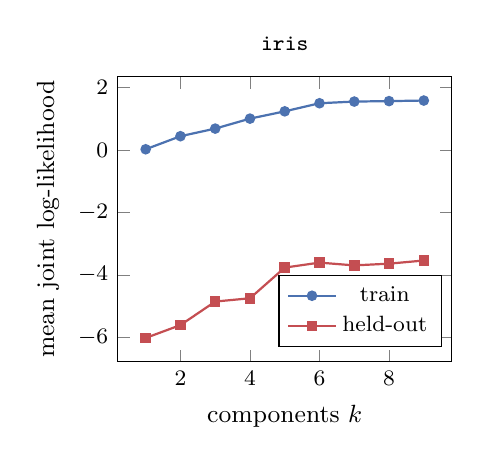
\begin{tikzpicture}
\begin{axis}[
  width=0.48\linewidth, height=5.2cm,
  xlabel={components $k$}, ylabel={mean joint log-likelihood},
  label style={font=\small}, tick label style={font=\footnotesize},
  legend style={font=\footnotesize, at={(0.97,0.05)}, anchor=south east},
  title={\footnotesize\texttt{iris}},
]
\addplot[cJPT, thick, mark=*, mark size=1.5pt] coordinates {(1,0.0220) (2,0.4403) (3,0.6834) (4,1.0028) (5,1.2356) (6,1.4950) (7,1.5486) (8,1.5634) (9,1.5812)};
\addplot[cBoost, thick, mark=square*, mark size=1.5pt] coordinates {(1,-6.0177) (2,-5.6053) (3,-4.8525) (4,-4.7465) (5,-3.7652) (6,-3.6057) (7,-3.6950) (8,-3.6394) (9,-3.5380)};
\legend{train, held-out}
\end{axis}
\end{tikzpicture}\hfill
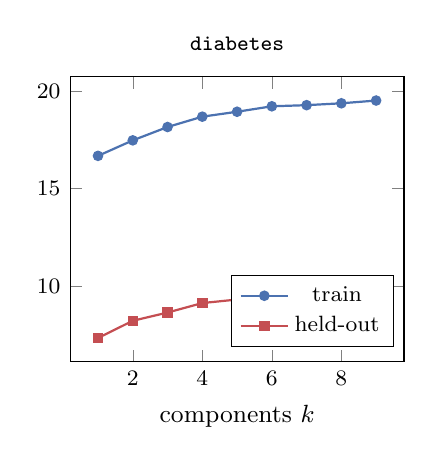
\begin{tikzpicture}
\begin{axis}[
  width=0.48\linewidth, height=5.2cm,
  xlabel={components $k$},
  label style={font=\small}, tick label style={font=\footnotesize},
  legend style={font=\footnotesize, at={(0.97,0.05)}, anchor=south east},
  title={\footnotesize\texttt{diabetes}},
]
\addplot[cJPT, thick, mark=*, mark size=1.5pt] coordinates {(1,16.6790) (2,17.4732) (3,18.1569) (4,18.6868) (5,18.9388) (6,19.2182) (7,19.2760) (8,19.3719) (9,19.5124)};
\addplot[cBoost, thick, mark=square*, mark size=1.5pt] coordinates {(1,7.3511) (2,8.2319) (3,8.6541) (4,9.1397) (5,9.3208) (6,9.6977) (7,9.8610) (8,10.0918) (9,10.1822)};
\legend{train, held-out}
\end{axis}
\end{tikzpicture}
\caption{\likeboost{} learning curves (single $75/25$ split, seed $0$):
mean joint log-likelihood of the round-$k$ prefix mixture. The train
curve is monotone by construction (non-improving rounds are rejected);
the held-out curve tracks it, i.e.\ the density gains generalise.
Prefix mixtures are recovered exactly by renormalising the first $k$
final weights (the Frank--Wolfe update scales them uniformly).}
\label{fig:lboost-curve}
\end{figure}

Figure~\ref{fig:lboost-curve} resolves the boosting trajectory of
\likeboost{} over rounds. The held-out curve follows the train curve
throughout the budget: on \texttt{iris} the mixture gains $2.5$ nats
per instance over nine components ($-6.02\to-3.54$), on
\texttt{diabetes} $2.8$ nats ($7.35\to10.18$), with no overfitting
visible---the acceptance rule (a component enters only if it improves
the training objective) and the $\mathcal O(1/t)$-shrinking
Frank--Wolfe step act as regularisers.

\begin{figure}[t]
\centering
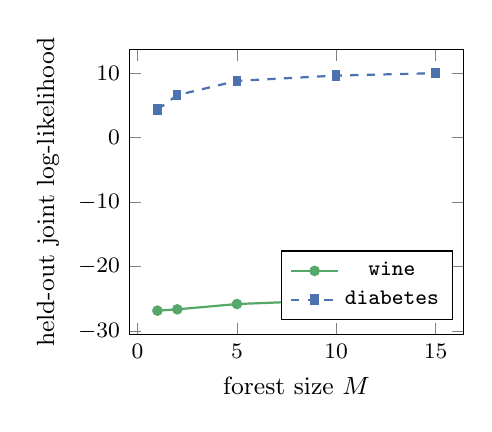
\begin{tikzpicture}
\begin{axis}[
  width=0.48\linewidth, height=5.2cm,
  xlabel={forest size $M$}, ylabel={held-out joint log-likelihood},
  label style={font=\small}, tick label style={font=\footnotesize},
  legend style={font=\footnotesize, at={(0.97,0.05)}, anchor=south east},
]
\addplot[cForest, thick, mark=*, mark size=1.5pt] coordinates {(1,-26.8230) (2,-26.6227) (5,-25.7998) (10,-25.2070) (15,-24.5802)};
\addplot[cJPT, thick, dashed, mark=square*, mark size=1.5pt] coordinates {(1,4.3677) (2,6.6008) (5,8.8125) (10,9.6410) (15,10.0040)};
\legend{\texttt{wine}, \texttt{diabetes}}
\end{axis}
\end{tikzpicture}\hfill
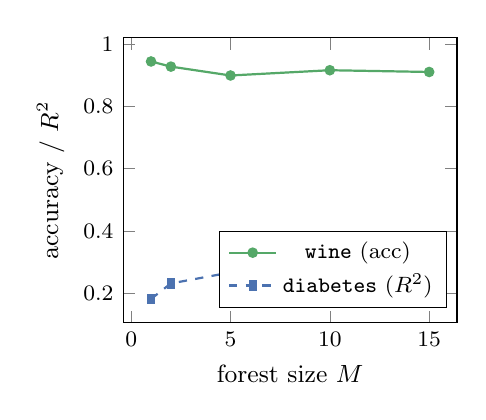
\begin{tikzpicture}
\begin{axis}[
  width=0.48\linewidth, height=5.2cm,
  xlabel={forest size $M$}, ylabel={accuracy / $R^2$},
  label style={font=\small}, tick label style={font=\footnotesize},
  legend style={font=\footnotesize, at={(0.97,0.05)}, anchor=south east},
]
\addplot[cForest, thick, mark=*, mark size=1.5pt] coordinates {(1,0.9440) (2,0.9275) (5,0.8990) (10,0.9159) (15,0.9103)};
\addplot[cJPT, thick, dashed, mark=square*, mark size=1.5pt] coordinates {(1,0.1818) (2,0.2315) (5,0.2667) (10,0.2412) (15,0.2484)};
\legend{\texttt{wine} (acc), \texttt{diabetes} ($R^2$)}
\end{axis}
\end{tikzpicture}
\caption{\jptforest{} quality vs.\ ensemble size $M$ ($5$-fold CV
means). $M{=}1$ is a single bootstrap tree. Most of the gain arrives by
$M\approx5$--$10$, the classic bagging saturation profile
(Prop.~\ref{prop:bag-var}).}
\label{fig:sweep}
\end{figure}

Figure~\ref{fig:sweep} varies the forest size. The density gain is
monotone in $M$ on \texttt{wine} ($-26.8$ at $M{=}1$ to $-24.6$ at
$M{=}15$) and saturates around $M{\approx}10$ on \texttt{diabetes}
($4.4\to10.0$). The predictive metrics move far less: $R^2$ peaks
already near $M{=}5$, and \texttt{wine} accuracy stays within one
fold-std of the single bootstrap tree throughout. Bagging JPTs buys
density quality first---consistent with Prop.~\ref{prop:bag-var},
whose variance-reduction argument applies to the density estimate
itself, not to any downstream decision rule.

% ---------------------------------------------------------------------------
\subsection{P2: predictive quality across the model family}
\label{sec:exp-pred}

\begin{table}[t]
\centering
\footnotesize
\setlength{\tabcolsep}{2.5pt}
\begin{tabular}{lrrrrrr}
\toprule
 & \multicolumn{3}{c}{generative (Bayes rule / posterior mean)} &
   \multicolumn{3}{c}{discriminative}\\
\cmidrule(lr){2-4}\cmidrule(lr){5-7}
dataset & \jpt & \jptforest & \likeboost & \jptboost & RF & HistGB\\
\midrule
\multicolumn{7}{l}{\emph{classification (accuracy)}}\\
iris & $0.940 \pm 0.039$ & $0.933 \pm 0.042$ & $0.947 \pm 0.016$ & $0.927 \pm 0.039$ & $0.940 \pm 0.025$ & $0.947 \pm 0.016$ \\
wine & $0.933 \pm 0.057$ & $0.916 \pm 0.055$ & $0.938 \pm 0.048$ & $0.938 \pm 0.020$ & $0.972 \pm 0.018$ & $0.972 \pm 0.018$ \\
breast\_cancer & $0.926 \pm 0.013$ & $0.931 \pm 0.006$ & $0.930 \pm 0.008$ & $0.951 \pm 0.016$ & $0.965 \pm 0.015$ & $0.970 \pm 0.012$ \\
digits & $0.751$ & $0.867$ & $0.751$ & $0.816$ & $0.971$ & $0.971$ \\
\midrule
\multicolumn{7}{l}{\emph{regression ($R^2$)}}\\
diabetes & $0.182 \pm 0.121$ & $0.241 \pm 0.105$ & $0.272 \pm 0.119$ & $0.445 \pm 0.132$ & $0.419 \pm 0.098$ & $0.398 \pm 0.141$ \\
abalone & $0.310 \pm 0.038$ & $0.342 \pm 0.040$ & $0.409 \pm 0.026$ & $0.541 \pm 0.030$ & $0.557 \pm 0.040$ & $0.531 \pm 0.030$ \\
\bottomrule
\end{tabular}
\caption{Predictive quality ($5$-fold CV mean~$\pm$~std;
\texttt{digits}: single split). The generative columns answer the
prediction as \emph{one} of many queries of a full joint; the
discriminative columns model only $P(y\mid\mathbf x)$.}
\label{tab:pred}
\end{table}

Table~\ref{tab:pred} places all six models side by side. Three
observations. First, the generative models---which answer the
prediction as one query among many of a full joint and never see a
discriminative objective---stay within a few points of the dedicated
discriminative models on the low-dimensional datasets. Second,
\jptboost{} behaves exactly as designed (\emph{P2}): it is the
strongest JPT-family predictor on both regression datasets ($0.445$ and
$0.541$ vs.\ $0.272$ and $0.409$ for the best generative variant) and
on \texttt{breast\_cancer}, and on \texttt{diabetes} it edges out
RandomForest---at the price of not being a joint. Third, the remaining
gap to RF/HistGB concentrates on \texttt{digits} and \texttt{wine},
where many weakly informative dimensions must be combined: the regime
where modelling the full joint is hardest and a purely conditional
model has the easier task.

% ---------------------------------------------------------------------------
\subsection{Ablation: Dirichlet-smoothed leaves}
\label{sec:exp-alpha}

Symbolic leaf distributions support additive (Dirichlet) smoothing
$P_\lambda(c)=(n_c+\alpha)/(n+\alpha|C|)$ via the \texttt{prior\_alpha}
setting. Comparing $\alpha{=}0$ against $\alpha{=}1$ on the
classification datasets, for single trees and forests: the held-out
joint log-likelihood shifts by at most $0.15$ nats (\texttt{iris}
forest, $-3.53\to-3.68$) and accuracy is unchanged to three digits on
every dataset. At these sample sizes the Dirichlet prior is a numerical
safety device---it bounds the \likeboost{} reweighting
$w\propto1/\bar p$ away from infinity when a symbolic leaf assigns a
class probability zero---rather than an accuracy knob.

% ---------------------------------------------------------------------------
\subsection{Discussion}

The experiments support all three claims and delimit their scope.
\emph{Cost.} The full query surface is not free: a single \jpt{} trains
in seconds, the ensembles in minutes ($M{=}10$ members cost roughly
$8$--$10\times$ a single tree), and scikit-learn's RandomForest is
$1$--$2$ orders of magnitude faster still. The value proposition of an
ensemble JPT is therefore not predictive rank per compute, but that
\emph{one} trained object answers likelihoods, arbitrary conditionals,
marginals, MPE and sampling besides the point prediction
(\S\ref{sec:inference}). \emph{Limitation.} \texttt{digits} marks the
boundary: bounded-support piecewise-linear joint densities over
${\gtrsim}40$ dimensions collapse to the smoothing floor on held-out
data, so likelihood-driven boosting stalls, while bagging still helps
predictively. Ensemble JPTs are best deployed at low-to-moderate
dimensionality---up to a few dozen mixed-type variables---which is
precisely where full-joint reasoning is typically wanted.
\emph{Division of labour.} Within the family the practical guidance is
simple: use \jptforest{} or \likeboost{} whenever the joint is needed
(they are interchangeable in quality; the boost gets there with fewer
components, the forest trains embarrassingly parallel), and
\jptboost{} when only $P(y\mid\mathbf x)$ matters and the last few
points of accuracy or $R^2$ justify giving the joint up.

% ===========================================================================
\section{Related work}
\label{sec:related}

\textbf{Density / generative boosting.}
Boosting density estimates as additive mixtures has a long lineage:
\citet{rosset2002boostdensity} boost density estimates by likelihood;
\citet{tolstikhin2017adagan} (AdaGAN) and \citet{grover2018boosted}
re-derive greedy additive generative mixtures; the convex-combination view
as Frank--Wolfe over the density simplex is made explicit by
\citet{cranko2019boosting}. Our Theorem~\ref{thm:fw} instantiates this for
tree-structured \emph{joint} densities with mixed variable types;
Proposition~\ref{prop:boost-valid} and \S\ref{sec:inference} supply what
the density-boosting literature usually leaves implicit---the validity of
the boosted density and the full inference calculus on it.
\textbf{Gradient boosting.} \citet{friedman2001gbm} and the
functional-gradient view of \citet{mason2000boosting} underlie \jptboost;
modern scalable implementations \citep{chen2016xgboost,ke2017lightgbm} are
the empirical yardstick. \textbf{Probabilistic / generative trees and
forests.} Bagging and random forests
\citep{breiman1996bagging,breiman2001rf}; density forests and generative
forests \citep{criminisi2012decision,correia2020joints}; sum-product
networks and probabilistic circuits \citep{poon2011spn,choi2020pc}, with
which a mixture of JPTs shares the tractable-mixture story: a mixture of
JPTs is a shallow probabilistic circuit whose sum unit has the members as
children, and our inference calculus (\S\ref{sec:inference}) is the
corresponding circuit semantics made concrete for the JPT query surface.
\textbf{JPTs.} The base formalism, its inference algorithms and the
single-tree conditioning construction are due to \citet{nyga2023jpt};
this paper supplies the ensemble layer on top of them.

% ===========================================================================
\section{Conclusions}
\label{sec:conclusion}

Ensembling JPTs is worthwhile only if it preserves what JPTs are for. We
therefore built both classic ensemble constructions---bagging
(\jptforest) and boosting (\likeboost)---as finite convex mixtures of
JPTs and proved the two properties a practitioner needs. First, both
ensembles are \emph{fully valid joint probability distributions}:
mixtures of self-normalised tree joints need no partition function
(Prop.~\ref{prop:mixture-closed}), and the boosted model, unrolled, is
itself such a mixture with explicit simplex weights at every round
(Prop.~\ref{prop:boost-valid})---with the boosting rule justified as
exact Frank--Wolfe ascent of the joint log-likelihood
(Thm.~\ref{thm:fw}). Second, \emph{every inference algorithm of the
single tree translates to the ensemble}: likelihood and all unconditional
queries distribute linearly over the members; conditional queries,
posteriors and expectations use the evidence-adjusted responsibilities
$r_m(e)\propto w_m P^{(m)}(e)$; conditioning returns again an ensemble
JPT, so the class is closed under evidence; MPE is answered by
member-wise candidate generation with exact mixture re-scoring, a lower
bound with natural exactness cases; and sampling is exact ancestral
sampling. Each formula corresponds to a method of the published
implementation and reduces to the single-tree semantics at $M=1$. The
discriminative \jptboost{} completes the family for pure point
prediction, with the loss of the joint stated as a property of additive
boosting rather than a limitation of the implementation. Together the
three classes let a user choose the ensemble by the queries they need,
never by what the ensemble happens to support.

% ===========================================================================
\begin{thebibliography}{99}
\setlength{\itemsep}{1pt}

\bibitem[Breiman(1996)]{breiman1996bagging}
L.~Breiman. Bagging predictors. \emph{Machine Learning}, 24(2):123--140,
1996.

\bibitem[Breiman(2001)]{breiman2001rf}
L.~Breiman. Random forests. \emph{Machine Learning}, 45(1):5--32, 2001.

\bibitem[Chen \& Guestrin(2016)]{chen2016xgboost}
T.~Chen and C.~Guestrin. XGBoost: A scalable tree boosting system. In
\emph{KDD}, 2016.

\bibitem[Choi et al.(2020)]{choi2020pc}
Y.~Choi, A.~Vergari, and G.~Van~den~Broeck. Probabilistic circuits: A
unifying framework for tractable probabilistic models. Technical report,
2020.

\bibitem[Correia et al.(2020)]{correia2020joints}
A.~Correia, R.~Peharz, and C.~de~Campos. Joints in random forests. In
\emph{NeurIPS}, 2020.

\bibitem[Cranko \& Nock(2019)]{cranko2019boosting}
Z.~Cranko and R.~Nock. Boosted density estimation remastered. In
\emph{ICML}, 2019.

\bibitem[Criminisi et al.(2012)]{criminisi2012decision}
A.~Criminisi, J.~Shotton, and E.~Konukoglu. Decision forests: A unified
framework for classification, regression, density estimation, manifold
learning and semi-supervised learning. \emph{Foundations and Trends in
Computer Graphics and Vision}, 7(2--3):81--227, 2012.

\bibitem[Frank \& Wolfe(1956)]{frankwolfe1956}
M.~Frank and P.~Wolfe. An algorithm for quadratic programming.
\emph{Naval Research Logistics Quarterly}, 3(1--2):95--110, 1956.

\bibitem[Friedman(2001)]{friedman2001gbm}
J.~H. Friedman. Greedy function approximation: A gradient boosting machine.
\emph{Annals of Statistics}, 29(5):1189--1232, 2001.

\bibitem[Grover \& Ermon(2018)]{grover2018boosted}
A.~Grover and S.~Ermon. Boosted generative models. In \emph{AAAI}, 2018.

\bibitem[Jaggi(2013)]{jaggi2013fw}
M.~Jaggi. Revisiting Frank--Wolfe: Projection-free sparse convex
optimization. In \emph{ICML}, 2013.

\bibitem[Ke et al.(2017)]{ke2017lightgbm}
G.~Ke, Q.~Meng, T.~Finley, et al. LightGBM: A highly efficient gradient
boosting decision tree. In \emph{NeurIPS}, 2017.

\bibitem[Mason et al.(2000)]{mason2000boosting}
L.~Mason, J.~Baxter, P.~Bartlett, and M.~Frean. Boosting algorithms as
gradient descent. In \emph{NeurIPS}, 2000.

\bibitem[Nyga et al.(2023)]{nyga2023jpt}
D.~Nyga, M.~Picklum, T.~Schierenbeck, and M.~Beetz. Joint Probability
Trees. \emph{arXiv:2302.07167}, 2023.

\bibitem[Poon \& Domingos(2011)]{poon2011spn}
H.~Poon and P.~Domingos. Sum-product networks: A new deep architecture. In
\emph{UAI}, 2011.

\bibitem[Rosset \& Segal(2002)]{rosset2002boostdensity}
S.~Rosset and E.~Segal. Boosting density estimation. In \emph{NeurIPS},
2002.

\bibitem[Tolstikhin et al.(2017)]{tolstikhin2017adagan}
I.~Tolstikhin, S.~Gelly, O.~Bousquet, et al. AdaGAN: Boosting generative
models. In \emph{NeurIPS}, 2017.

\end{thebibliography}

\end{document}
